\documentclass[twoside,12pt]{article}
\usepackage{fancyhdr}
\usepackage[margin=1in]{geometry}
\usepackage{hyperref}
\usepackage{minitoc}
\usepackage{pdfpages}
\usepackage{secure-page-numbers}
\usepackage{tocloft} % for special ToC formatting; see gross below

\newcommand{\setfootershift}[1]{\lhead{} \rhead{} \cfoot{\vspace{#1} \colorbox{white}{\ \thepage\ }}}
% USAGE: \addproceedings{intro}
\newcommand{\addproceedings}[1]{
	% Align cryptographic page numbers on their own line in main ToC.
	% Pretty gross, huh? Looks nice tho.
	\cftsetpnumwidth{37em}
	\renewcommand\cftsecleader{\newline\cftdotfill{\cftdotsep}}
	\renewcommand\cftsubsecleader{\newline\cftdotfill{\cftdotsep}}
	\renewcommand\cftsubsubsecleader{\newline\cftdotfill{\cftdotsep}}
	\renewcommand\cftparaleader{\newline\cftdotfill{\cftdotsep}}
	%\renewcommand\cftsecpagefont{\bfseries} % already this way but if you wanna change it
	\renewcommand\cftsubsecpagefont{\itshape}

	\renewcommand{\contentsname}{#1}
	\tableofcontents
	\pagebreak}
% USAGE: \addtrack{number}{name}
\newcommand{\addtrack}[2]{
	\cleardoublepage
	\begin{center}
	#1 \\
	\section*{#2}
	\addcontentsline{toc}{section}{#1: #2}
	\end{center}
	% More grossness to remove page numbers in track ToCs
	% OMG IT FINALLY WORKS SHIP IT
	\renewcommand\cftsecleader{\cftdotfill{\cftnodots}}
	\renewcommand\cftsubsecleader{\cftdotfill{\cftnodots}}
	\renewcommand\cftsubsubsecleader{\cftdotfill{\cftnodots}}
	\renewcommand\cftparaleader{\cftdotfill{\cftnodots}}
	% Pretty much copied from tocloft.sty, only the "#1" is removed.
	\renewcommand{\cftsubsecfillnum}[1]{%
		{\cftsubsecleader}\nobreak
		\makebox[1.5em][\cftpnumalign]{\cftsubsecpagefont}\cftsubsecafterpnum\par}
	\renewcommand{\cftsubsubsecfillnum}[1]{%
		{\cftsubsubsecleader}\nobreak
		\makebox[1.5em][\cftpnumalign]{\cftsubsubsecpagefont}\cftsubsubsecafterpnum\par}
	\renewcommand{\cftparafillnum}[1]{%
		{\cftparaleader}\nobreak
		\makebox[1.5em][\cftpnumalign]{\cftparapagefont}\cftparaafterpnum\par}
	\secttoc}
% USAGE: \addpaper{title}{author}{keywords}{filename}{page number vertical shift}
\newcommand{\addpaper}[6]{
	\setfootershift{#5}
	\rhead{#6}
	\includepdf[pages=-,pagecommand={\thispagestyle{fancy}},addtotoc={1,subsection,1,{#1},{title:#4},1,subsubsection,4,{#2},{author:#4},1,paragraph,4,{Keywords: #3},{keywords:#4}},picturecommand={\rhead{}}]{./papers/#4}}
% USAGE: \addreview{filename}{page number vertical shift}
\newcommand{\addreview}[2]{
	\setfootershift{#2}
	\includepdf[pages=-,pagecommand={\thispagestyle{fancy}}]{./reviews/#1}}

\renewcommand{\headrulewidth}{0pt}
\renewcommand{\stctitle}{}
\renewcommand{\thepage}{\roman{page}}
\renewcommand{\thesection}{}
\renewcommand{\thesubsection}{\arabic{subsection}}

\setcounter{tocdepth}{2}

\mtcsetdepth{secttoc}{4}
\mtcsetpagenumbers{*}{off}
\mtcsetrules{*}{off}
\dosecttoc

\setfootershift{0cm}

\begin{document}
\pagenumbering{shahash}
\includepdf[pagecommand={\thispagestyle{plain}}]{titlepage}
\includepdf[pagecommand={\thispagestyle{plain}}]{copyright-page}
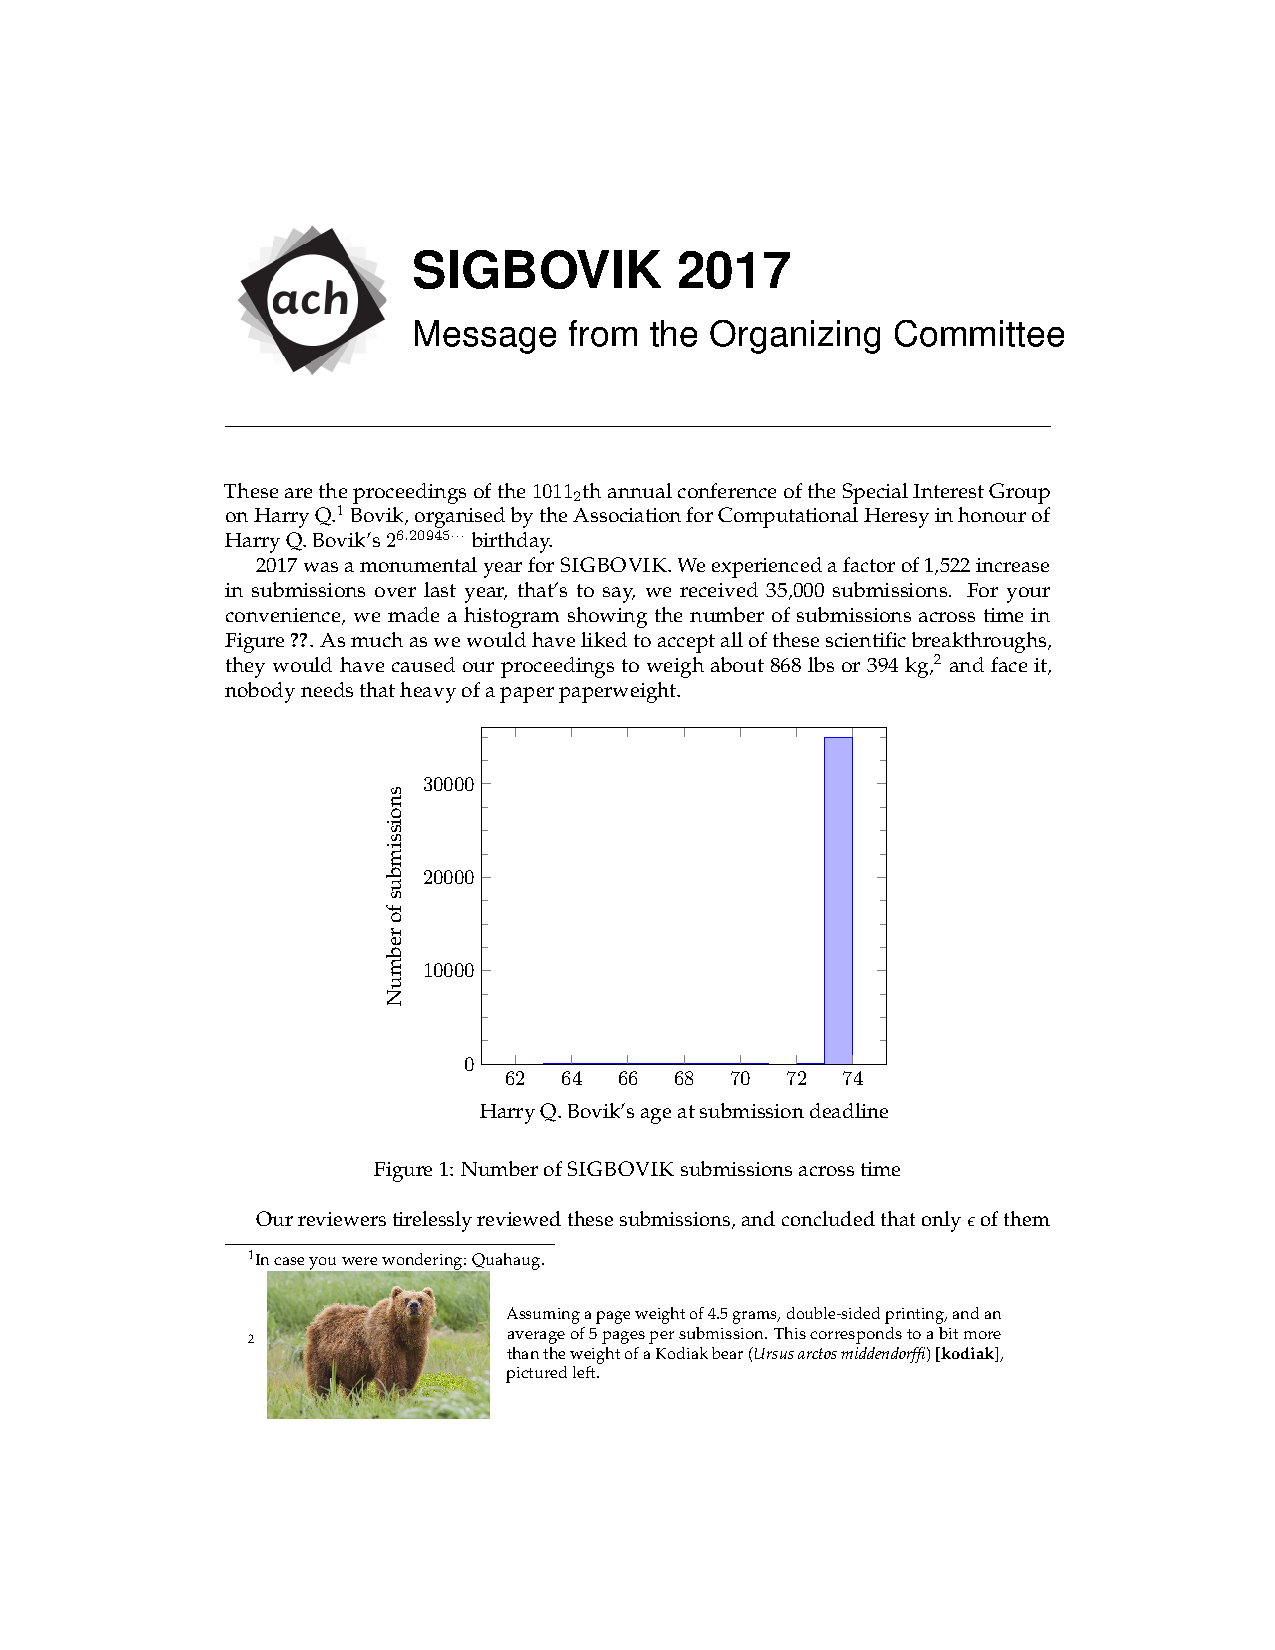
\includepdf[pages=-,pagecommand={\thispagestyle{plain}}]{message-from-committee}

\addproceedings{ToC About Proceedings! Have We Got Papers for You!}

\addtrack{Half-track}{Crypticography}
\addpaper
	{Cryptographically secure page numbering in \LaTeX}
	{William Gunther and Brian Kell}
	{cryptography, hashing, LaTeX, macros, page numbers, security, SHA-256}
	{SIGBOVIK_2016_paper_18}
	{0cm}
	{
\includegraphics[width=1in]{eval}}
\addreview{paper18eval}{-1.45cm}
\addpaper
	{Random seed generation}
	{Alexander R.\ Frieder}
	{random, seed, encryption, complexity, am, I, even, supposed, to, fill, this, out, what, amI, doing, ?}
	{SIGBOVIK_2016_paper_1}
	{0cm}
	{}

\addtrack{Full track}{Safety Schools of Thought}
\addpaper
	{Reducing the trusted constituent base with the LCF approach: Hillary, the next 700 elections}
	{Brandon Bohrer, Sol Boucher, and Jos Valdivida}
	{illogical, logic, Hillary, elections, congressional, fuckery, robustness, constituents, unrest, pork-barreling, curtain-closing}
	{SIGBOVIK_2016_paper_25}
	{0cm}
	{}
\addpaper
	{Unprl: Nuprl proof re-evaluation logic}
	{Ryan Kavanagh}
	{proof assistant, Nuprl, The Wizard of Oz, artificial artificial intelligence}
	{SIGBOVIK_2016_paper_11}
	{0cm}
	{}
\addpaper
	{Type-safe friends will never hurt you}
	{Brandon Bohrer}
	{friendship logic, friends, office mates, Cwelf}
	{SIGBOVIK_2016_paper_9}
	{-2cm}
	{}
\addreview{review9}{0cm}

\addtrack{Rototiller track}{Overcomplexity Theory}
\addpaper
	{The computational complexity of Chinese and Italian noodle making}
	{Daniel M.\ Berry and Luisa Mich}
	{algorithm, Chinese mian, computational complexity, Italian pasta, noodle}
	{SIGBOVIK_2016_paper_2}
	{0cm}
	{}
\addreview{paper2review}{0cm}
\addpaper
	{Which ITG stepcharts are turniest?}
	{Ben Blum}
	{in, the, groove}
	{SIGBOVIK_2016_paper_12}
	{0cm}
	{
\includegraphics[width=1in]{eval}}
\addreview{paper12eval}{-1.45cm}

\addtrack{Lamb track}{Languages: Human and... Inhuman}
\addpaper
	{Lambda Doge: A digital canine language}
	{Joshua Suereth}
	{lambda calculus, doge, programming languages}
	{SIGBOVIK_2016_paper_15}
	{0cm}
	{}
\addpaper
	{Making the theoretical possible: the untyped $\lambda$-calculus in C++}
	{Jim McCann}
	{lambda, c++, c++11}
	{SIGBOVIK_2016_paper_23}
	{0cm}
	{}
\addpaper
	{A shortmantout}
	{David Renshaw and Jim McCann}
	{portmanteausteritycoon, hotshots, carthartichokes, sadjustment}
	{SIGBOVIK_2016_paper_13}
	{0cm}
	{}

\addtrack{Footpath track}{HyperLink to DnD}
\addpaper
	{The glEnd() of Zelda}
	{Dr.\ Tom Murphy VII Ph.D.}
	{small keys, boss keys, dungeon keys}
	{SIGBOVIK_2016_paper_16}
	{-1.1cm}
	{}
\addpaper
	{Student success and sorrow: The determination of professor alignment and its effects on students}
	{D.\ Daly and E.\ Binns}
	{professors, academia, alignment}
	{SIGBOVIK_2016_paper_24}
	{-1.9cm}
	{}

\addtrack{Garbage track}{Reduce, Reuse, Recycle}
\addpaper
	{PRESS RELEASE: FOR IMMEDIATE WORLDWIDE RELEASE}
	{Nicholas Fudala and Chester Francis}
	{editors note, this didnt seem very important, so we sat on it for 2 years, with love, the ach committee for retrocausal publication impact}
	{SIGBOVIK_2016_paper_17}
	{0cm}
	{}
\addpaper
	{Pittsburgh is a grid}
	{Stefan Muller}
	{Pittsburgh, grids, unnecessary integrals, computational geography}
	{SIGBOVIK_2016_paper_10}
	{-0.3cm}
	{
\includegraphics[width=1in]{eval}}
\addreview{paper10eval}{-1.35cm}

\addtrack{Oversized track}{How (Over)fitting}
\addpaper
	{Reordering snacks is effective and just}
	{Dr.\ Tom Murphy VII Ph.D.}
	{snacking, permutations, comestability theory}
	{SIGBOVIK_2016_paper_8}
	{-1.2cm}
	{}
\addpaper
	{0-order Non-linear ordinary differential equations}
	{Oscar I.\ Hernandez and Daniel J.\ Packer}
	{ordinary differential equations, non-linear, nonhomo}
	{SIGBOVIK_2016_paper_5}
	{0cm}
	{}
\addpaper
	{Deep spreadsheets with ExcelNet}
	{David Fouhey and Daniel Maturana}
	{deep learning, Excel, LibreOffice, convolutional neural network, spreadsheet}
	{SIGBOVIK_2016_paper_21}
	{0cm}
	{}
\addpaper
	{Sniffing for meaning: Defining and maximizing the signal-to-nose ratio}
	{Josh Cox}
	{signal, nose, ratio, sniff, smell, scent}
	{SIGBOVIK_2016_paper_22}
	{0cm}
	{}

\addtrack{Cattle track}{Higher-order Research}
\addpaper
	{On the topic of "um..."}
	{Timothy J.\ Parenti}
	{um, best, paper}
	{SIGBOVIK_2016_paper_20}
	{-0.55cm}
	{}
\addpaper
	{SMACK: When research in algorithms goes around in circles}
	{Patrick Lin and Weishuang Linda Xu}
	{algorithms, collider, particle physics}
	{SIGBOVIK_2016_paper_4}
	{-2cm}
	{}
\addpaper
	{A look into the mind of the modern graduate student via telephonic obfuscation}
	{Erik Harpstead \textit{et al.}}
	{comestibility theory, telephonic obfuscation, computer human interaction}
	{SIGBOVIK_2016_paper_6}
	{0cm}
	{}
\addpaper
	{Dinner grant renewal request}
	{From Dr.\ Angus McNabb III to Jim McCann}
	{dinner, dog pictures, naps, napping, nap time, sleeping}
	{SIGBOVIK_2016_paper_14}
	{0cm}
	{}
\addpaper
	{Ode to reviewer two}
	{Anonymous}
	{ode, double-blind review, false politeness, landslide}
	{SIGBOVIK_2016_paper_7}
	{0cm}
	{}
\addreview{review-bestpaper}{0cm}

\end{document}
